\documentclass[a4paper, 12pt, twoside]{article}
\usepackage[a4paper, top=2.5cm, bottom=2.5cm, left=3.5cm, right=2.5cm]{geometry}

\usepackage[MeX]{polski} 
\usepackage[T1]{fontenc}
\usepackage[utf8]{inputenc}
\usepackage{times}
% Polish language pack
\usepackage{indentfirst}
% Indent first paragraph after section header
\usepackage{graphicx}
% Enhanced support for graphics
\graphicspath{{images/}}
% Set default graphics path
\usepackage{mathptmx}
% Use Times as default text font, and provide maths support
\usepackage{amsmath}
%  AMS mathematical facilities
\usepackage{tikz}
% Create PostScript and PDF graphics
\usepackage{hyperref}
% Extensive support for hypertext
\usepackage[final]{pdfpages}
% Include PDF documents
\usepackage{afterpage}
% Execute command after the next page break
\usepackage{titlesec}
% Select alternative section titles
\usepackage{microtype}
% Ad­just­ment of in­ter­word spac­ing and ad­di­tional kern­ing, etc.
\usepackage{enumitem}
% Control layout of itemize, enumerate, description
\usepackage{caption}
\usepackage{subcaption}
% Customising captions
\usepackage{listings}
% Typeset source code listings
\usepackage{chngcntr}
% Change the resetting of counters
\counterwithin{figure}{section}
% Ustawia numerację obrazków

\lstset{
   frame=single,
   numbers=none,
   captionpos=b,
   tabsize=4,
   basicstyle=\footnotesize\ttfamily,
   breaklines=true,
   inputencoding=utf8,
   extendedchars=true,
   literate={ą}{{\k{a}}}1
             {Ą}{{\k{A}}}1
             {ę}{{\k{e}}}1
             {Ę}{{\k{E}}}1
             {ó}{{\'o}}1
             {Ó}{{\'O}}1
             {ś}{{\'s}}1
             {Ś}{{\'S}}1
             {ł}{{\l{}}}1
             {Ł}{{\L{}}}1
             {ż}{{\.z}}1
             {Ż}{{\.Z}}1
             {ź}{{\'z}}1
             {Ź}{{\'Z}}1
             {ć}{{\'c}}1
             {Ć}{{\'C}}1
             {ń}{{\'n}}1
             {Ń}{{\'N}}1
}
% Ustawia styl listingów

\frenchspacing
% Ustawia francuski spacing tekstu
\linespread{1.5}
% Ustawia odstęp linii na 1.5cm
\newcommand\tab[1][0.5cm]{\hspace*{#1}}
% Ustawia skrót na akapit 1cm do komendy \tab
\titleformat*{\section}{\fontsize{14}{12}\selectfont\bfseries}
\titleformat*{\subsection}{\fontsize{12}{12}\selectfont\bfseries}
% Ustawia styl nagłówków rozdziałów i podrozdziałów

\hypersetup{
    colorlinks,
    citecolor=black,
    filecolor=black,
    linkcolor=black,
    urlcolor=black
}
% Ustawia kolory linków

\newcommand\blankpage{%
	\null
    \thispagestyle{empty}%
    \newpage}
% Ustawia komendę do wyświetlania pustej strony

\pdfinfo{
   /Author (Krzysztof Dragan)
   /Title  (Aplikacja internetowa do wyszukiwania połączeń lotniczych)
   /CreationDate (\today)
   /Keywords (Praca;dyplomowa;inzynierska;modyfikacja;stfc)
}
% Ustawianie metadanych pliku PDF
  
% --------------------------------------------
% ------------ Początek dokumentu ------------
\begin{document}
\counterwithin{lstlisting}{section}
% Zmienia numerację listingu na numer aktualnego rozdziału
% --------------------------------------------
% -------------- Strona tyłułowa -------------
\afterpage{\blankpage}
\begin{titlepage}
	\centering
		
	{\fontsize{16pt}{12pt}\selectfont
		\MakeUppercase{\textls[150]{Politechnika Świętokrzyska}}\\ 
		Wydział Elektrotechniki, Automatyki i Informatyki \par}
		
	\vspace{0.1cm}
	\hrule
	\vspace{2.5cm}
		
	{\fontsize{14pt}{12pt}\selectfont
		\scshape\textbf{Krzysztof Dragan}}\\
	Numer albumu: 083524
	\\
	\vfill
	{\fontsize{20pt}{12pt}\selectfont
		\bfseries Aplikacja internetowa\\ do wyszukiwania połączeń lotniczych\par}
	\vspace{1cm}
	{\fontsize{14pt}{12pt}\selectfont
		Praca dyplomowa inżynierska\\
		na kierunku Informatyka\\ \par}
	\vspace{7cm}
	\hfill	Opiekun pracy dyplomowej:\par
	\hfill dr inż. Arkadiusz \textsc{Chrobot}\par
	\hfill Katedra Systemów Informatycznych
	\vfill
	Kielce \the\year \par
\end{titlepage}

% --------------------------------------------
% ------------------ Zadanie -----------------
\afterpage{\blankpage}
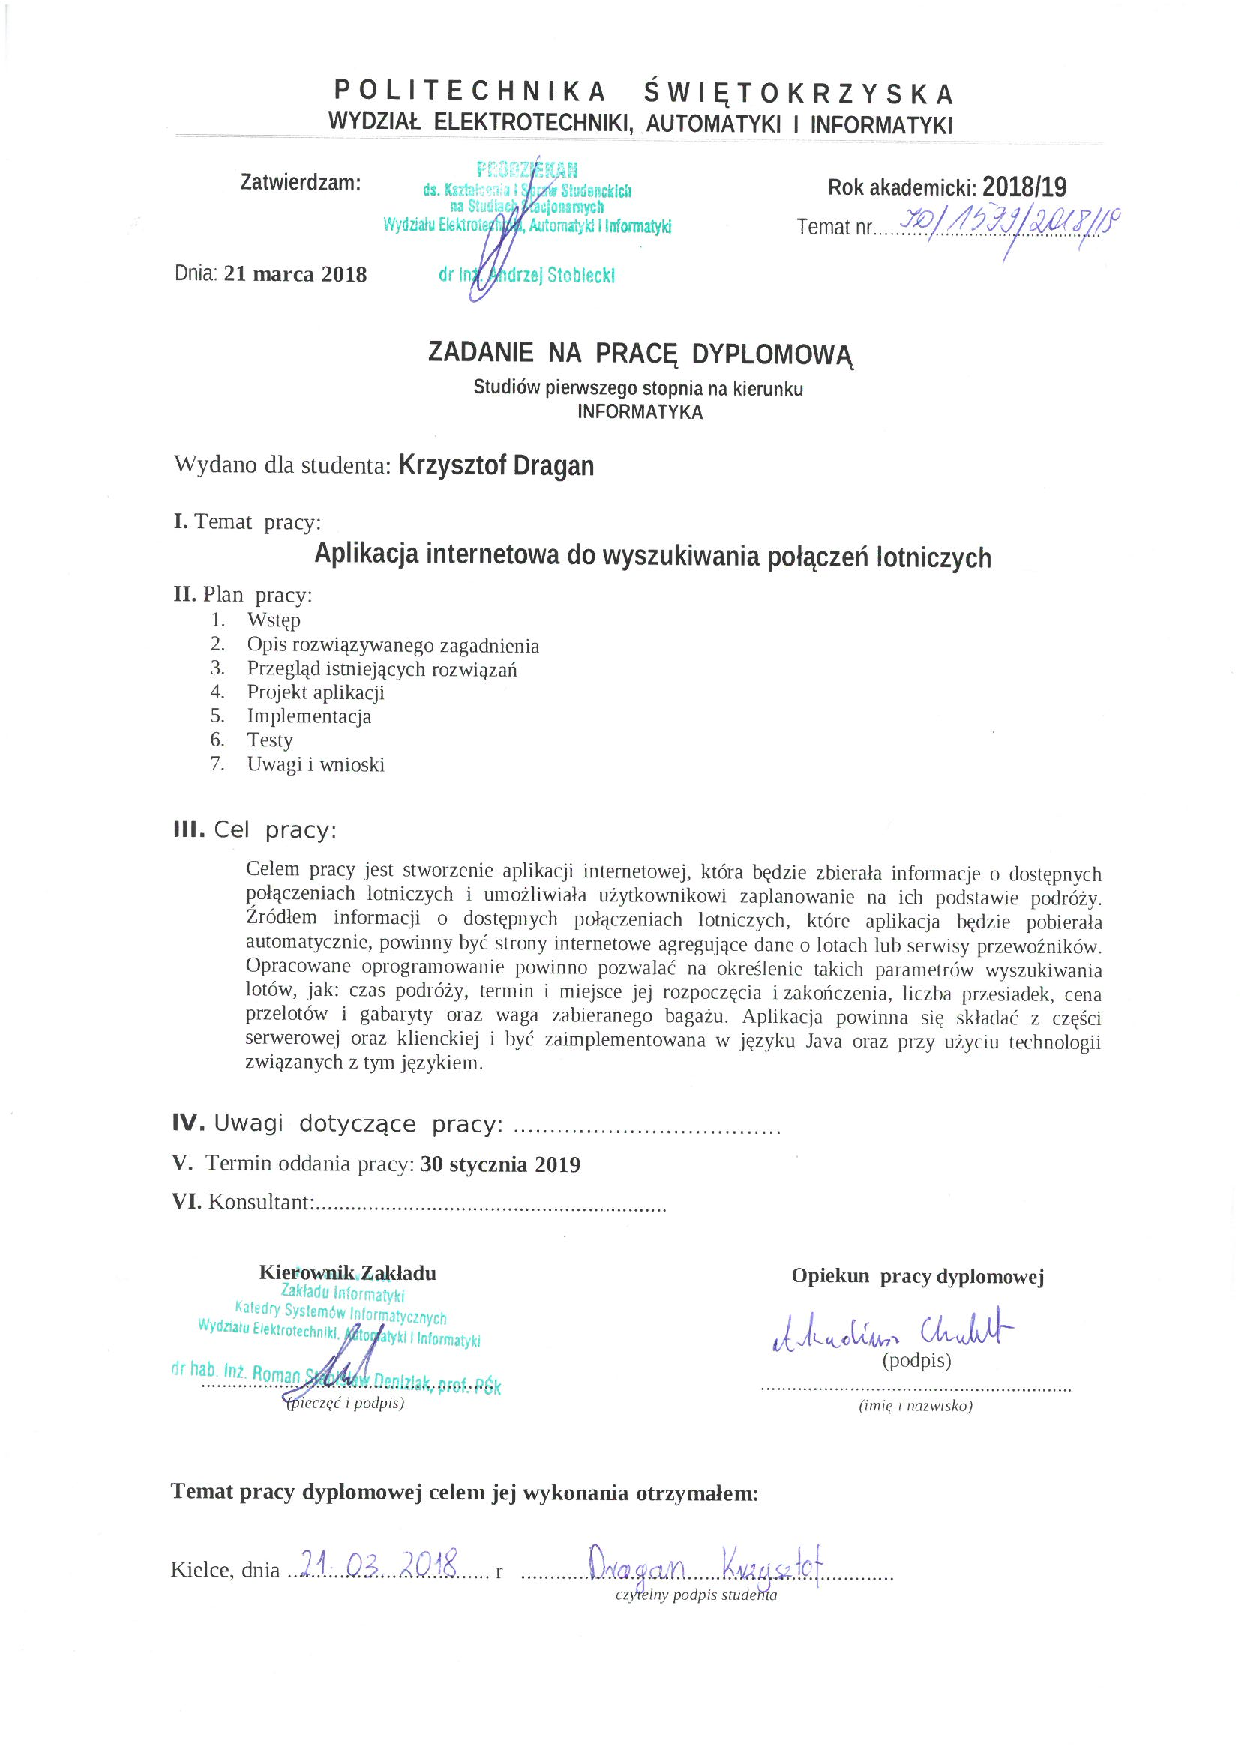
\includepdf[pages=-]{docs/zadanie.pdf}

% --------------------------------------------
% ---------------- Oświadczenie --------------
\afterpage{\blankpage}
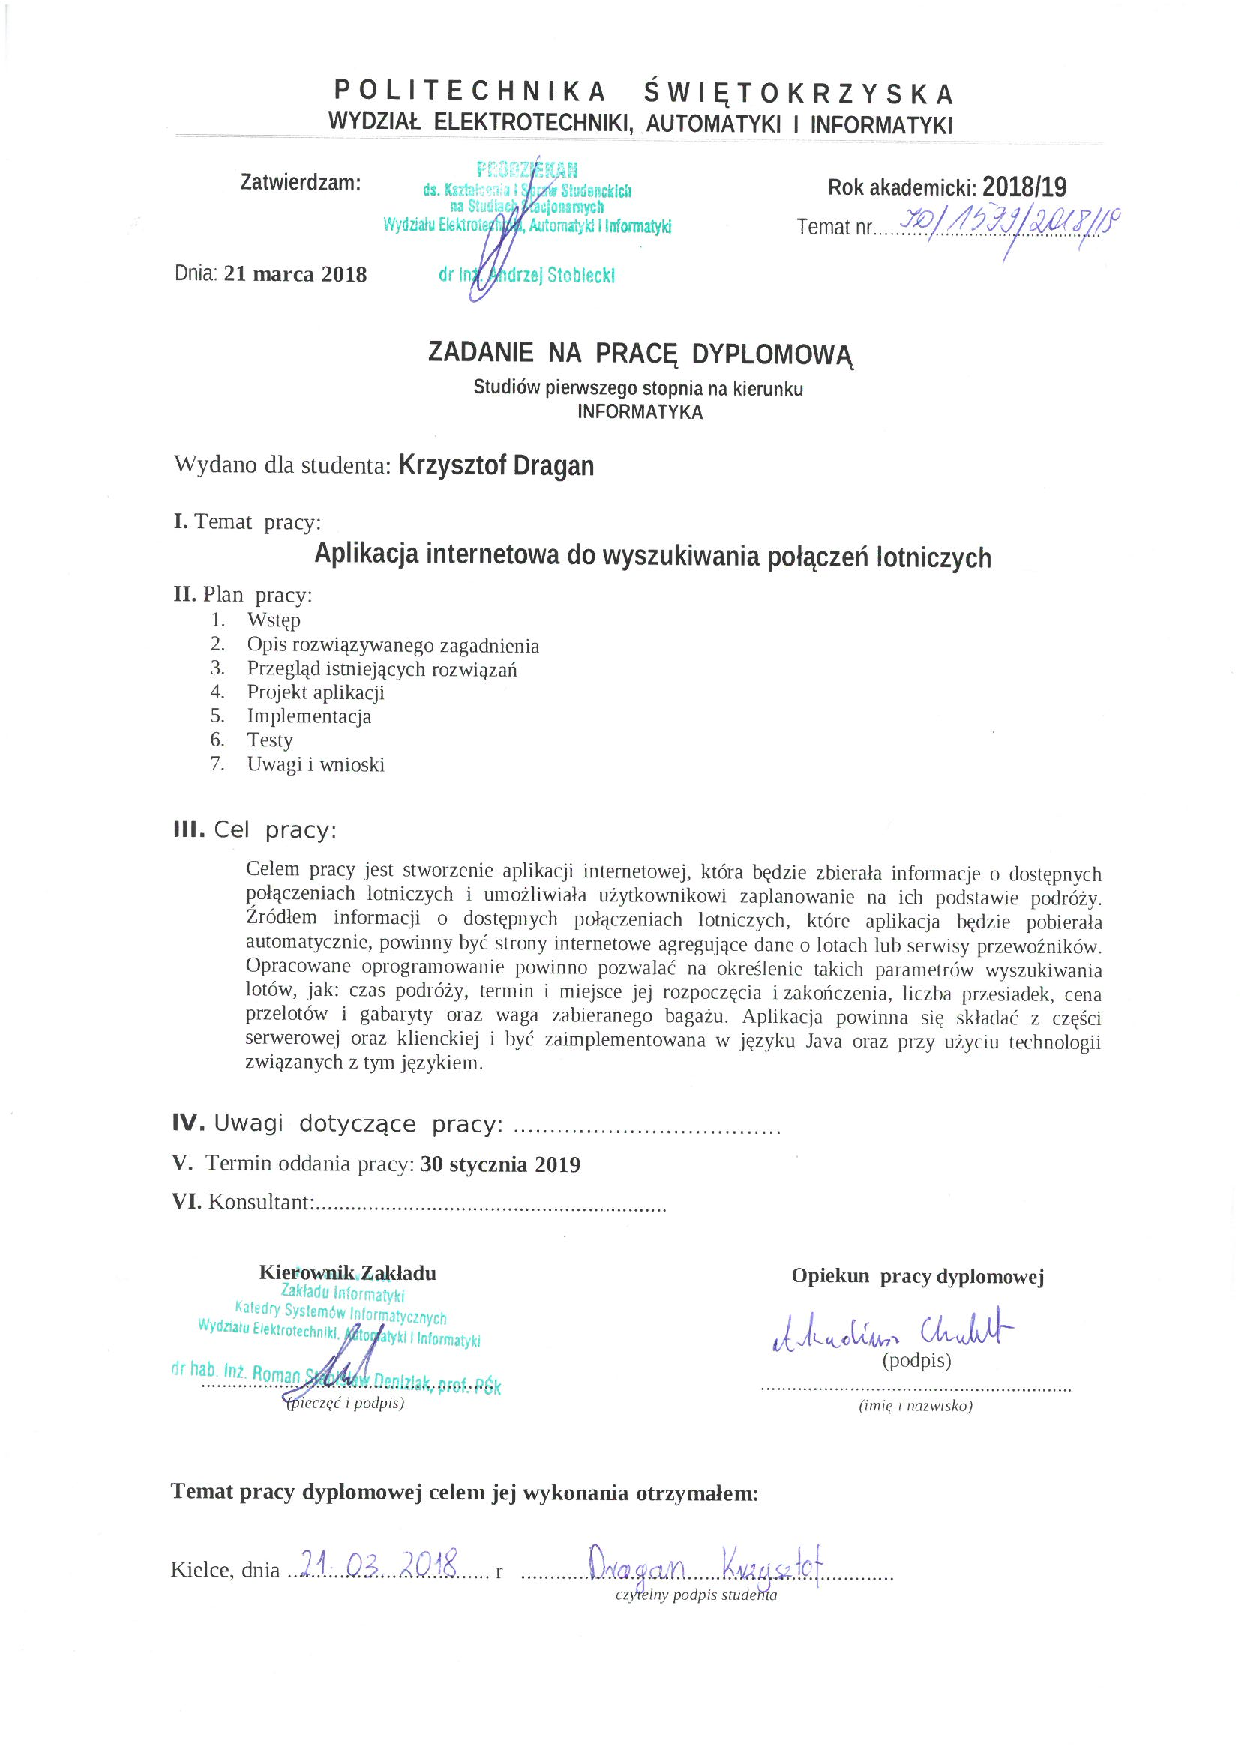
\includepdf[pages=-]{docs/zadanie.pdf}  

% --------------------------------------------
% --------------- Streszczenie ---------------
\newpage
\thispagestyle{empty}
\begin{center}
	{\fontsize{14pt}{12pt}\selectfont
		\textbf{Aplikacja internetowa do wyszukiwania połączeń lotniczych}}
\end{center}

\begin{flushleft}
	{\fontsize{14pt}{12pt}\selectfont
		\textbf{Streszczenie}}\\
	\vspace{1cm}
\tab Celem niniejszej pracy było opracowanie aplikacji internetowej która pozwoliłaby na wyszukiwanie połączeń lotniczych korzystając z danych zawartych na stronach internetowych przewoźników bądź z innych centr danych. Aplikacja została podzielona na część kliencką oraz serwerową. Klient został napisany przy użyciu technologii Angular 6, natomiast część serwerowa w technologii Java 10. W pracy znajduje się opis architektury stworzonej aplikacji, modułu wyszukiwania połączeń lotniczych a także zagadnień teoretycznych związanych z projektowaniem interfejsu użytkownika dla przeglądarki internetowej.
\end{flushleft}
\vspace{0.5cm}
Słowa kluczowe: Java, Angular 6, REST, programowanie obiektowe, protokół HTTP, programowanie funkcyjne

\vspace{1.5cm}

\begin{center}
	{\fontsize{14pt}{12pt}\selectfont
		\textbf{A web application to search for flight connections}}
\end{center}

\begin{flushleft}
	{\fontsize{14pt}{12pt}\selectfont
		\textbf{Summary}}\\
	\vspace{1cm}
\tab The purpose of thesis was to build a web application, which will be able to search flight connections using data included on air websites or others data sources. Application was divided into two parts: client and server. Client was implemented using technology of Angular 6, whereas server in Java 10 technology. Description of architecture built application, module of air connections searching and theoretical issues related to building user interface for web application are included in this thesis. 
\end{flushleft}
\vspace{0.5cm}
Keywords: - Java, Angular 6, REST, Object Oriented Programming, HTTP Protocol, Functional Programming
\afterpage{\blankpage}

% --------------------------------------------
% ---------------- Spis Treści ---------------
\renewcommand{\contentsname}{Spis treści}
\newpage
\pagenumbering{arabic}
\setcounter{page}{9}
% Ustawia numerację strony od aktualnej na numer 9
\tableofcontents

% --------------------------------------------
% ------------------- Wstęp ------------------
\newpage
\section{Wstęp}

\end{document}